\section{Test mit zusätzlichen Addiererklauseln} % 211 - 291
\label{sec:test_234}

Im Test aus Abschnitt \ref{sec:test_modul} wurden die modulspezifischen Klauseln getestet, jedoch zusätzliche Klauseln für den Addierer weggelassen.
Das betrifft die Klauseln aus Tabelle \ref{fig:additional_clauses_add}, die in diesem Test separat getestet werden.
Die Ergebnisse sind in Abbildung \ref{fig:data_add} dargestellt. Die Testlaufzeit beider Varianten sind mehr als doppelt so hoch und bei der
Anzahl der unterschiedlichen Lösungen lässt sich keine Veränderung erkennen.
\begin{figure}[!h]
  \centering
  \begin{minipage}[c]{0.45\textwidth}
  \begin{flushleft}Gesamtdauer ohne XOR: 410:59:52\end{flushleft}
  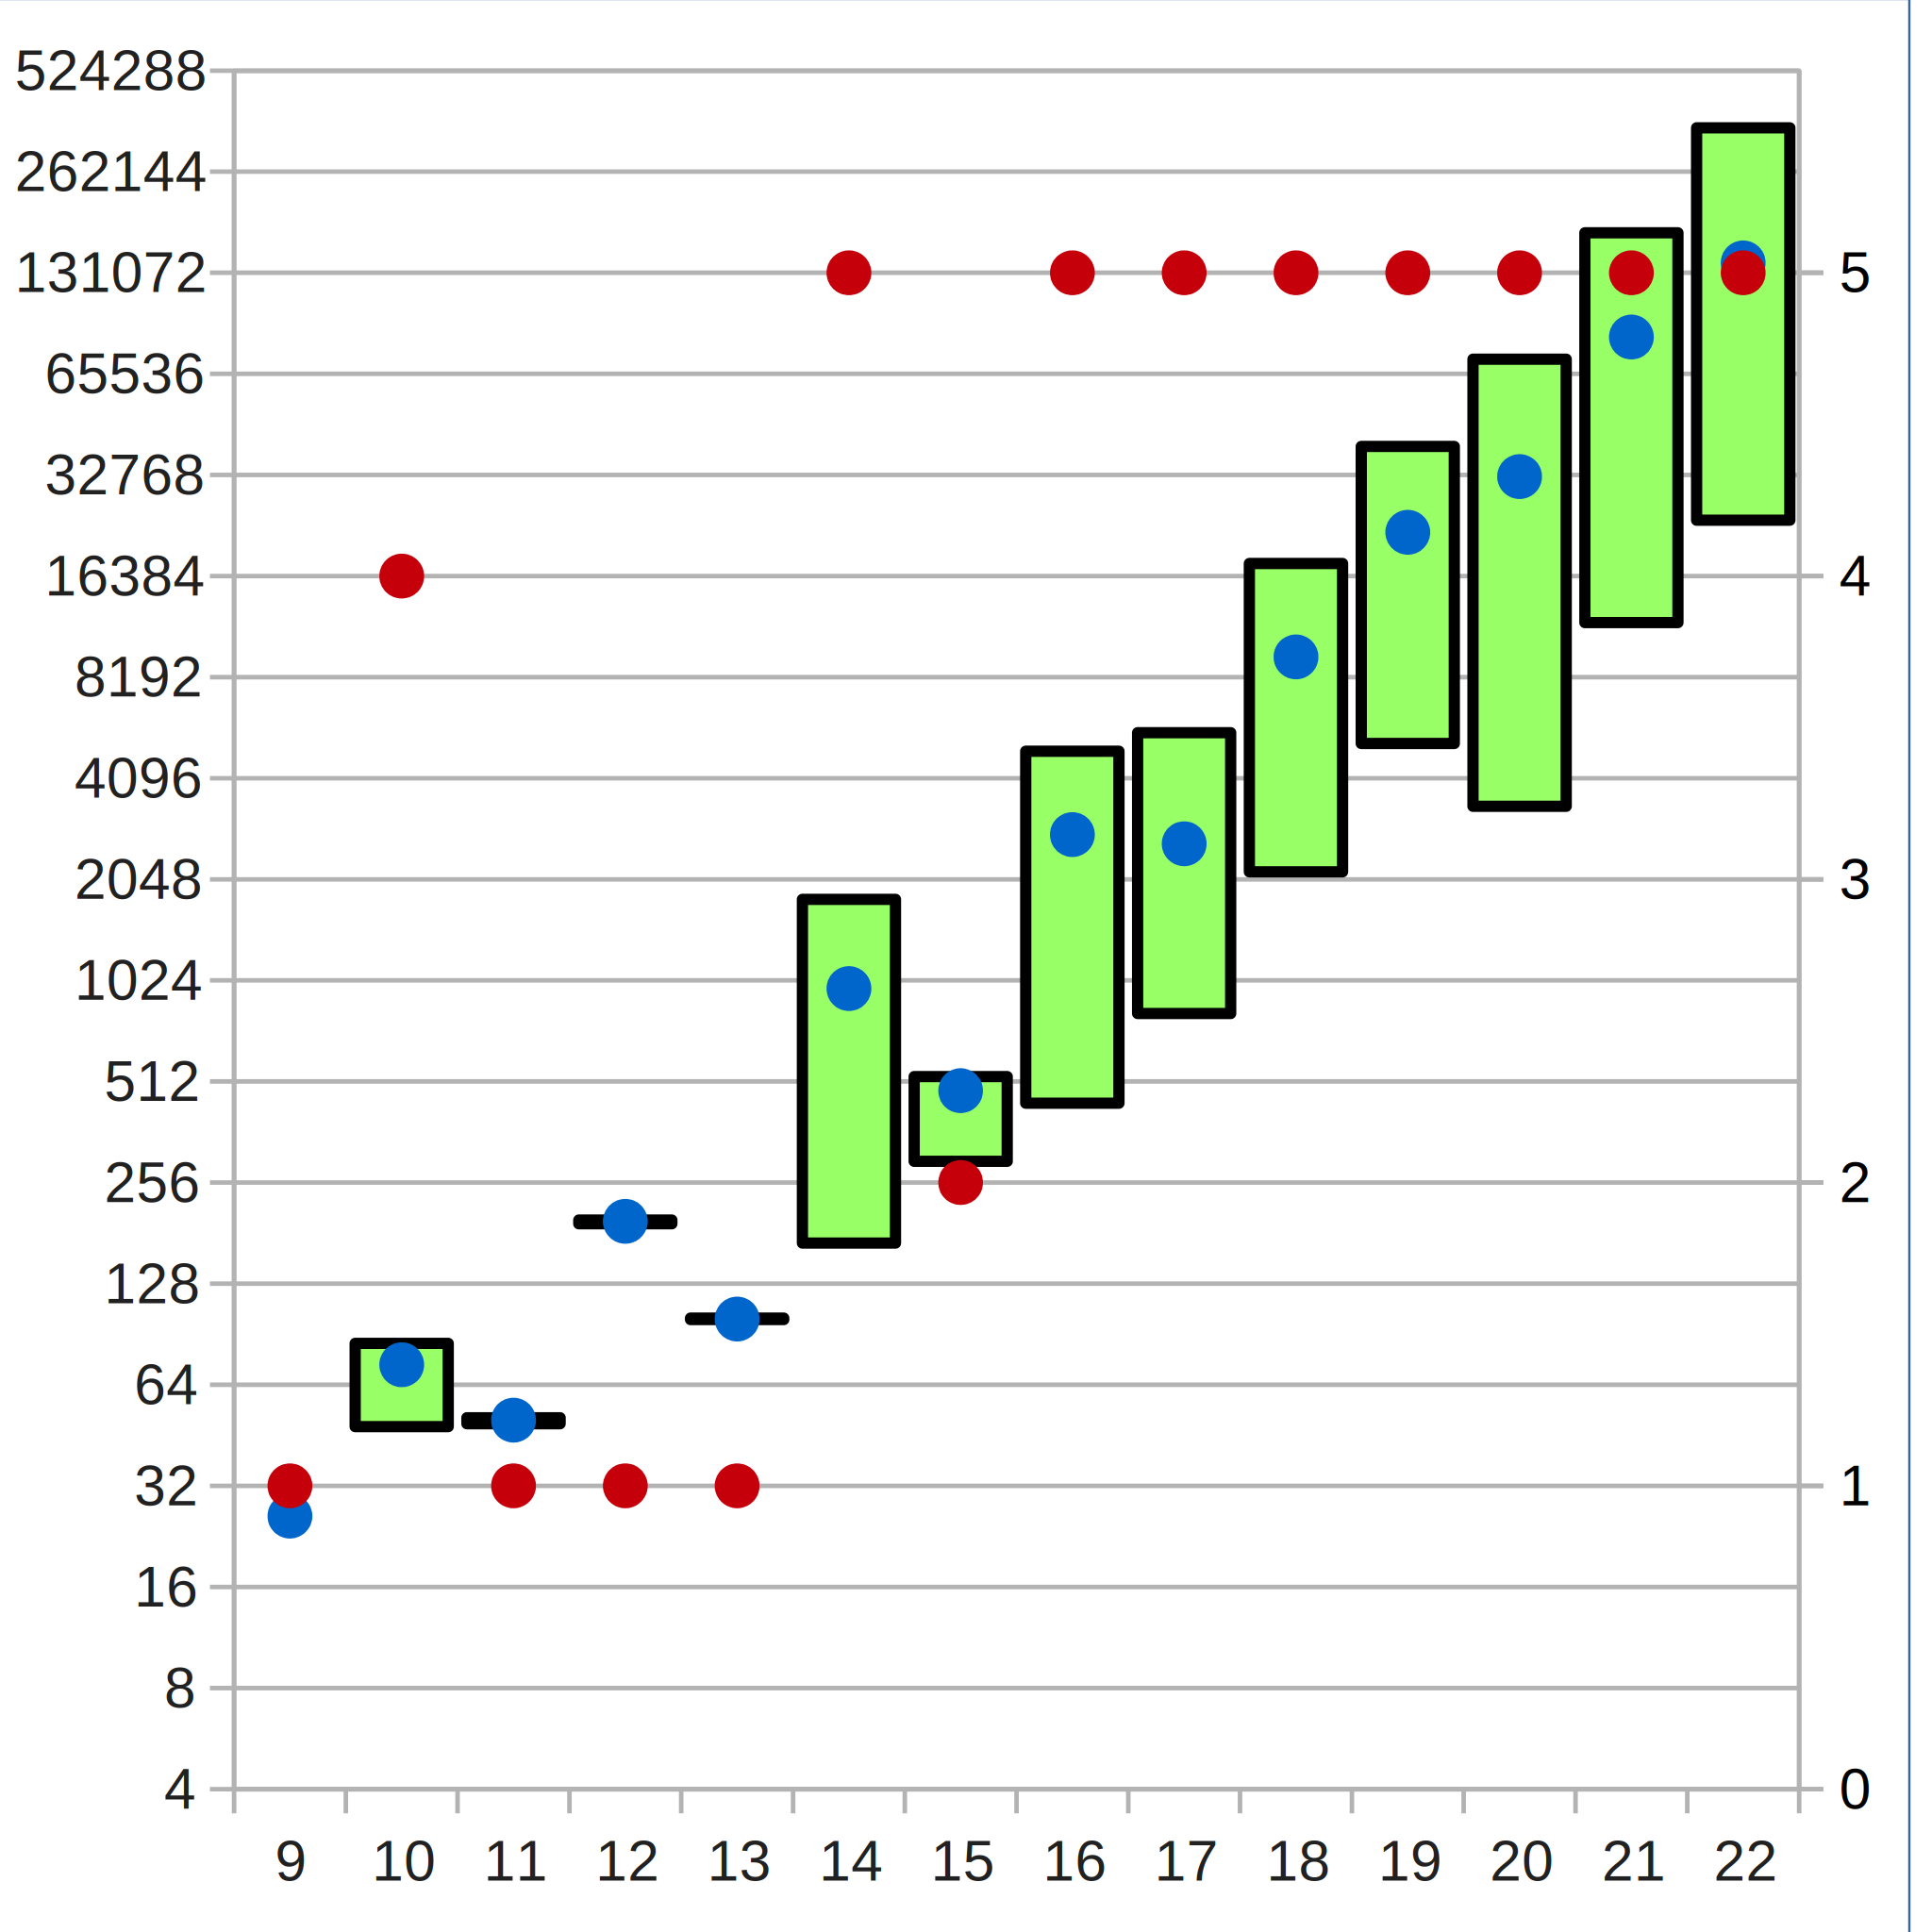
\includegraphics[scale=0.55]{images/data_add_knf}
  \end{minipage}
  \begin{minipage}[c]{0.09\textwidth}
  ~~
  \end{minipage}
  \begin{minipage}[c]{0.45\textwidth}
  \begin{flushleft}Gesamtdauer mit XOR: 491:53:48\end{flushleft}
  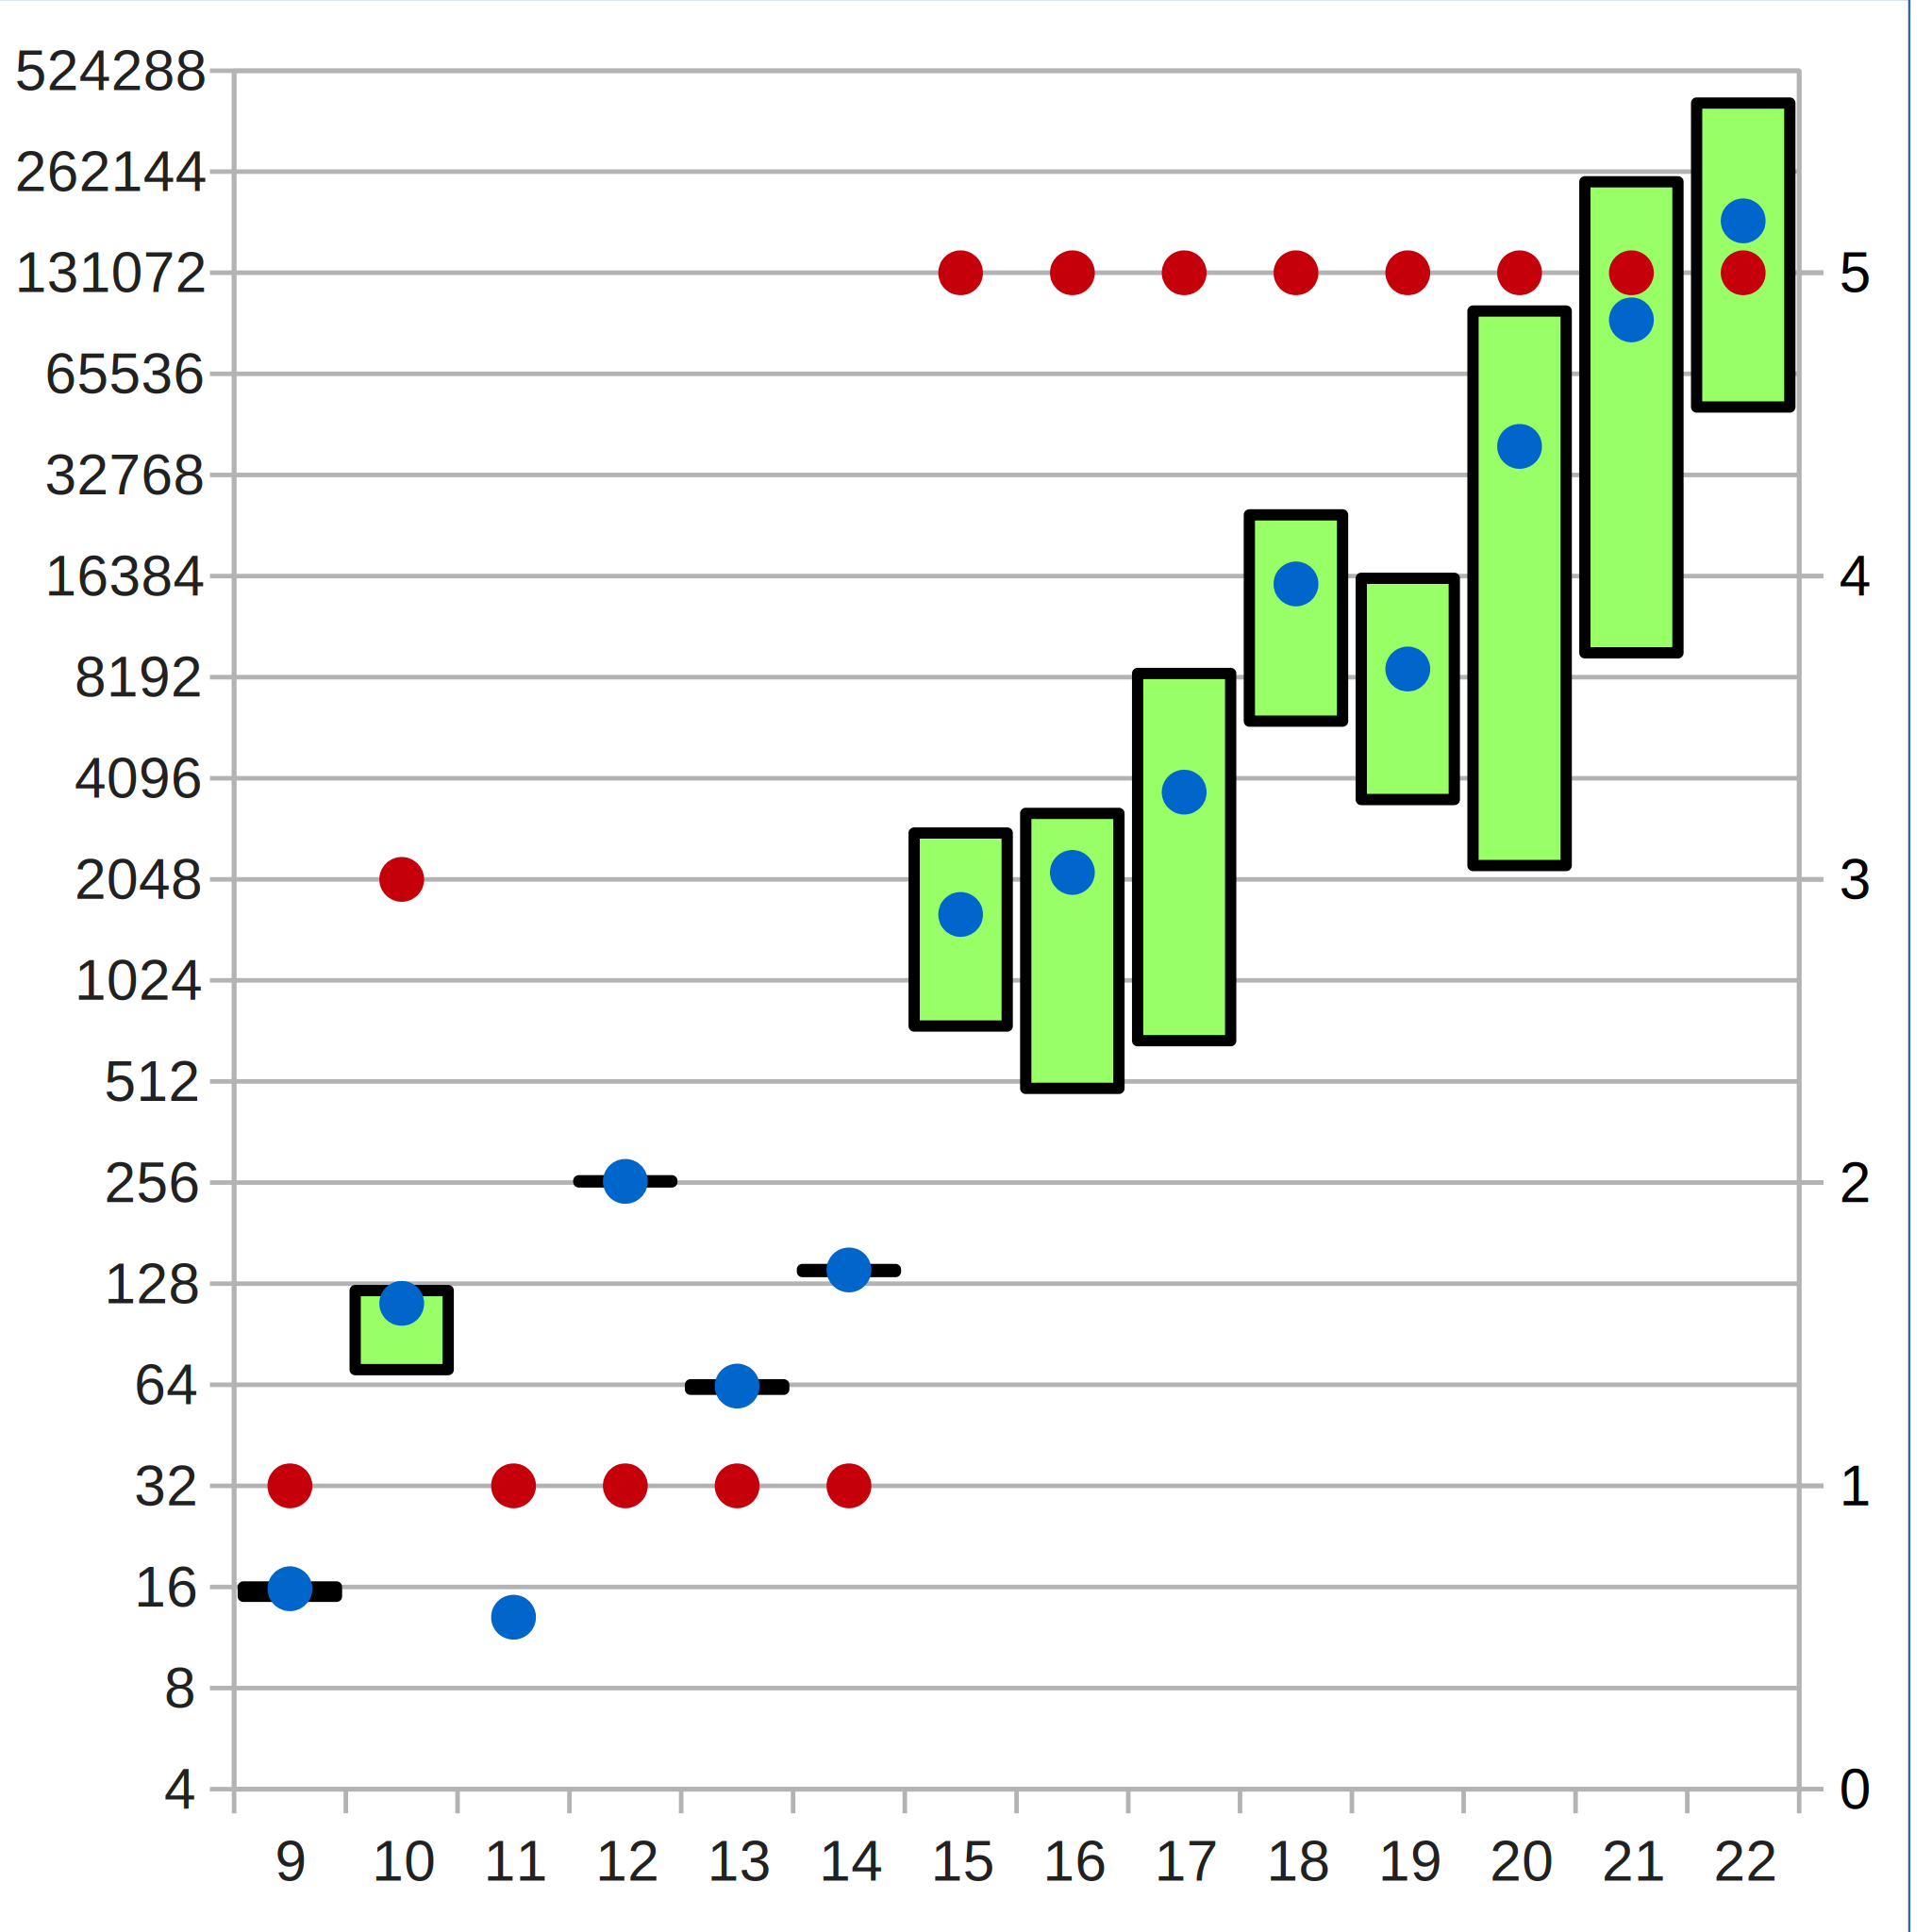
\includegraphics[scale=0.55]{images/data_add_xor}
  \end{minipage}
  \caption{Ergebnisse mit zusätzlichen Addiererklauseln}
  \label{fig:data_add}
\end{figure}